
\chapter{Results} \label{c:results}

This chapter collects results of the most relevant tests performed on the application. 

First, an assessment of the overall effectiveness of the optimiser is presented. A brief analysis of computational performance is also given, alongside an estimation of the time requirements in correlation to the problem size. Finally, the choice of parameters for the Genetic Algorithm is discussed.

\section{Corridor Performance Optimisation} \label{r:kpi}
Several tests were performed on randomly generated 8 junction corridors, with sections of variable length between the controlled junctions and varying demand flows accessing the corridor and leaving it at each intersection.

The tests presented in this section are concerned with the optimisation phase: models represent the corridor sub-networks, as would be produced for the rapid execution of the DNL algorithm. Traffic flow profiles entering the cordon arcs and hence the corridor, as well as turn rates, are assumed pre-calculated in the DTA phase as detailed in section \ref{s:rollingtre}.

This section considers several optimisation runs performed on the same representative 8-junction corridor, since the process is not deterministic and it is important to assess the consistency of results as well as their quality. The evolution of solution fitness as driven by each of the corridor performance functions is shown relative to the initial value, which invariably corresponds to one of the slack bandwidth \emph{geometrical} solution variants used to prime the GA population as described in section \ref{s:poppriming}.

The results presented demonstrate how the proposed method can significantly improve the corridor performance in relation to all of the proposed metrics, although each of them is more or less susceptible to optimisation under different traffic conditions.

\pagebreak
\subsection{Stable Subcritical Demand}

To assess performance under \emph{sub-critical} traffic conditions, several optimisation runs are performed while ensuring that no corridor link is subjected to demand flows that exceed its capacity after the reduction imposed by the effective green time, which is taken to be constant for the present application, i.e. $\saturation_{a} = \frac{\flowratio_a}{\gamma_a} < 1 \; \forall a \in \corridor$.

Performance improvements over the simple geometrical solution are shown in Figure \ref{f:subcrit}. 

\fig{h}{PIX/RES/cold_subcrit.png}{f:subcrit}{Evolution of cost function values for subcritical flows and high side flows between 10\% and 30\% : solid lines in the foreground represent the average trend of the corresponding lighter sets in the background.}{width=0.75\textwidth}

It is also interesting to note that if the traffic conditions are close to the theoretical premises of the simple bandwidth maximisation approach (i.e. if congestion does not significantly affect travel times and side flows are almost negligible with respect to the main corridor flow) the solutions found by the optimiser, even with a \emph{completely random} initial population, never stray far from the geometrical solution, as shown in Figure \ref{f:similar}, and are \emph{identical} in case of no relevant side flows.

\fig{htbp}{PIX/RES/shapes_thinner.png}{f:similar}{Comparison of the average trajectory of a \emph{green wave front} under sub-critical conditions and side flows of varying entity in relation to the total flow through each junction. The trajectory is the path a hypothetical vehicle would have to follow to drive through the start of every green phase along the corridor, obtained from the average results of ten runs for each scenario starting from random solutions (vertical bars show the standard deviation). With increasing side flows, offsets are adjusted to meet the side-flow platoons, and the main green wave must move more slowly, as visible from the steeper segments on the T-D diagram.}{width=0.8\textwidth}

This is an important empirical confirmation of the system's stability and coherence with its theoretical background. As side flows increase, the optimal solutions diverge further and further from the simple spatio-temporal alignment of the green phases. This is only to be expected: vehicles that enter from cordon links reach the next junction ahead of those travelling along the corridor; as their number grows they start swaying the cost function significantly, so that the genetic algorithm will favour synchronisation patterns that minimise their discomfort.

The onset of the green phase at each junction is hence anticipated to meet the platoon coming from the side road, so that it may incur as little stops as possible and leave little or no queue behind for the main flows to run into. The effect is visible in Figure \ref{f:similar} where the green wave trajectories (which can never travel faster than free-flow speed) are shown to slow down to meet the onset of the next green phase.


\subsection{Stable Supercritical Demand}
The foremost advantage of simulation-based heuristic optimisation is the possibility to search for better signal timings even if the traffic conditions are so distant from the ideal bandwidth maximisation scenario that making sensible \emph{a priori} assumption about platoon arrival and queue discharge times becomes practically impossible.

The proposed optimiser was therefore extensively tested under \emph{super-critical} traffic conditions, with relevant side flows entering the corridor during the main red phase and several arcs operating above their saturation capacity ($\saturation \simeq 1.3 \pm 0.1$). Under these conditions, queues are \emph{bound} to form on all such arcs (considerably affecting travel times) and a relevant fraction of the vehicles is not travelling through all junctions in sequence: simple geometrical solutions become completely inadequate.

The first scenario considered reproduces the optimisation of a time window during which high demand volumes rapidly enter an otherwise tranquil network, and aims to assess the capacity of the optimiser to keep corridor performance indicators in check. Figure \ref{f:coldstart} confirms that compared to the geometrical solutions that would serve the uncongested scenario, optimised plans can considerably reduce the number of stops and the growth of queues on short arcs. 

\fig{htb}{PIX/RES/cold_super.png}{f:coldstart}{Evolution of cost function values for the optimisation window containing the onset of high demand flows. Solid lines in the foreground represent the average trend of the corresponding lighter sets in the background.}{width=0.7\textwidth}

It appears that queue management is most susceptible to early convergence into locally optimal solutions, as shown by the evident fork in the relevant values across the sample of optimisation runs, which for the test scenario presented in Figure \ref{f:coldstart} represents a 66\% difference in gains over the starting solution between the worst and best cases; in every instance, however, gains are relevant and above 15\% of the initial cost. 

The average travel time may \emph{seem} less sensitive to optimisation, due to the relatively small improvement in the relevant cost function. However, if the metric is inverted for readability as shown on the left-hand side of Figure \ref{f:speedimpro}, it is plain that the effect is due to the average speed being high to begin with: in fact, the optimiser is able to improve the performance with respect to the maximum bandwidth solution by a respectable 3 km/h, almost as well as in the case of sub-critical demand.

\fig{htbp}{PIX/RES/speed_impro2.png}{f:speedimpro}{Improvements in progression speed, averages and standard deviations corresponding to the scenarios presented in Figures \ref{f:subcrit}, \ref{f:coldstart} (left) and \ref{f:rollingstart} (right). The average user speed can be maintained effectively and consistently as long as the corridor does not collapse under sustained flows above capacity, after which gains become almost irrelevant and the optimiser behaviour is less reliable.}{width=\textwidth}

The second test scenario envisions an already heavily congested corridor with standing queues on most arcs, as the optimiser would inevitably face either during normal operation at peak hours or upon being switched back on after a down time. 

It is plain to see from Figure \ref{f:rollingstart} that while the standing queues mean that little can be done to avoid further stops, the \emph{queue length} can be managed rather effectively and consistently, with improvements between 6\% and 8\% shown across all tests. The same gains are obtained with respect to travel times, which being the inverse of the average speed across the subcritical and hypercritical portions of each arc are directly correlated with the queue length, as discussed in section \ref{s:quel}.

Predictably, these large relative improvements are not as striking in terms of speed, which would be low in any case due to congestion as shown by the right-hand side of Figure \ref{f:speedimpro}. Nevertheless, they represent a positive reduction in the time lost by users in peak-hour traffic, e.g. for the test corresponding to Figure \ref{f:rollingstart} users travelling the whole corridor would shave about two minutes off a seventeen minute trip in the best case scenario.

\fig{htb}{PIX/RES/roll_super.png}{f:rollingstart}{Evolution of cost function values for an already congested corridor experiencing sustained flows above capacity. Solid lines in the foreground represent the average trend of the corresponding lighter sets in the background.}{width=0.9\textwidth}


\section{Computational Performance} \label{res:performance}
All tests presented in this section were performed on a 3.4 GHz Intel\textregistered Core\texttrademark i7-2600 CPU running up to 8 parallel threads on four processor cores. The computation times already proved adequate for \emph{large} real world applications and entirely sufficient for smaller networks, as shown in Table \ref{t:performance}.

Sizing of the optimisation look-ahead window must chiefly account for the lower bound imposed by the minimum time required by the optimiser to reach satisfying results, as discussed in Chapter \ref{c:optimiser}.

With the optimal population size determined as in section \ref{r:popsize} and the performance goal set to the best gains obtained across other tests (during which no time limitation was imposed), it was ascertained that corridor optimisation is indeed possible within the desired rolling-horizon time window of 10 minutes.

\begin{table}[h]
\caption{\textsc{Optimisation Performance and Computation Times}} \label{t:performance}
\begin{center}
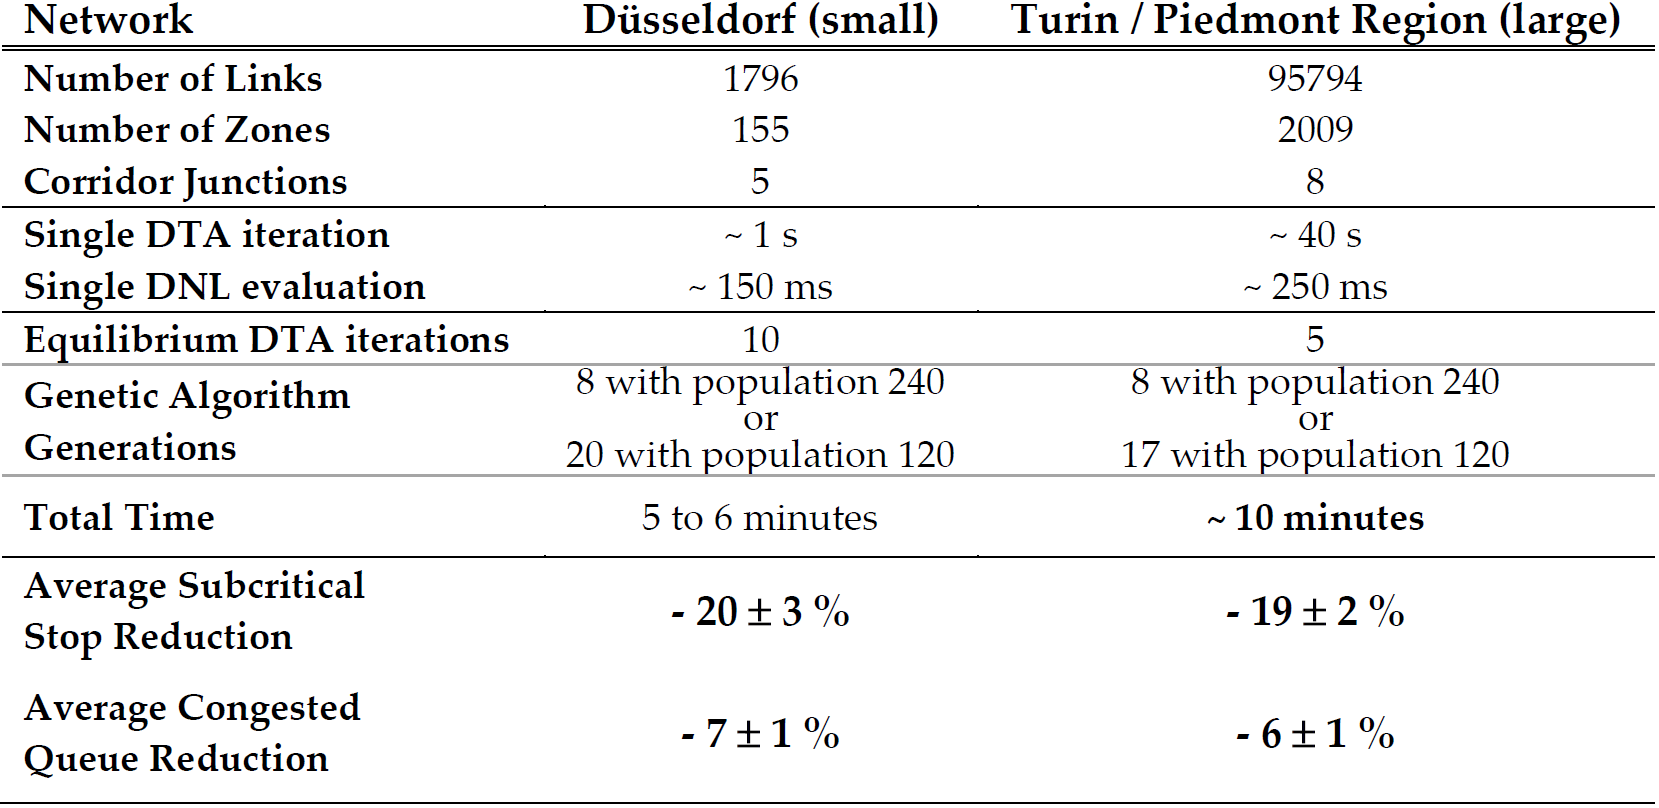
\includegraphics[width=0.9\textwidth]{PIX/RES/perftable.png}
\end{center}
\end{table}


\section{Bi-directional Slack Bandwidth}
slackband section \ref{s:slackband}.

\todo{Demonstrate how the two way corridor actually performs much better with the slack band solution:
\begin{itemize}
\item make graph
\end{itemize}
}

\fig{htbp}{PIX/undoguy.png}{f:slackvhardres}{ Bar graph with 70-30\% main:return optimised slackband vs maxband , SsShMain, QsQhMain ... TsThReturn}{width=0.4\textwidth}

Slack Bandwidth section \ref{s:slackband} show it is much better than reg band for similar "progression" objectives (travel times) for a two-way band max problem with weights proportional to flows. \todo{rant about how novel this is.}

\section{Algorithm Parameters}
This section presents results of the preliminary studies aimed at determining an optimal choice of parameters for the Genetic Algorithm.

\subsection{Population Priming} \label{s:poppriming}
Stochastic search methods are extremely sensitive to the choice of initial conditions. To speed up convergence and obtain better results, the present application initialises the genetic algorithm population using a geometrical solution (illustrated in section \ref{s:slackband}) that aims to align the green phases on the corridor so as to maximise the chance of driving through the longest possible distance without encountering a red light.

As discussed in section \ref{s:seeding}, it is necessary to ensure that the more \emph{informed} starting point does not imply a much narrower-sighted search of the solution space, ultimately leading to early convergence and sub-optimal results. The problem is clearly \emph{not} independent of the population size, and priming becomes at the same time more useful \emph{and} more risky for smaller and smaller populations (which might be preferable from the computational point of view).

The choice of \emph{partial} population priming with slack band solutions made for the present application is the consequence of the results shown in Figure \ref{f:priming}. For a reasonably sized population (see section \ref{r:popsize}) the best results are obtained by priming \emph{half} of the initial individuals with the geometrical solution, while the rest are generated randomly. 

\fig{htbp}{PIX/RES/priming.png}{f:priming}{Average cost function evolution arising from different population priming methods (sample size 20 optimisation runs for each scenario). Different problems favour geometrical solutions (if congestion and side flows are negligible, see left-hand side) or an initially random, unbiased population (as traffic conditions become less predictable, see right-hand side).
A mix of the two performs practically as well as either in its best case, but across the whole range of test scenarios.}{width=\textwidth}

As expected, geometrical priming is particularly beneficial if the traffic conditions are close to the uncongested free flowing state on large sections of the corridor, while as delays and side flows increase an entirely random population performs better thanks to the more thorough and unbiased search of the solution space, but in a practical application the call could not be made a-priori without some complicated selection logic.

However, provided with a mixed initial population, the Genetic Algorithm can effectively select those \emph{traits} of the geometrical solutions that apply to some corridor section, while including the diversity brought about by random solutions to yield near-optimal results across the whole range of tests performed with varying congestion and side flow levels.

\subsection{Population Size} \label{r:popsize}
In general, a larger population is able to preserve more diversity and avoid early convergence, ultimately reaching better results, but as the number of individuals increases so does the time required to complete one full generation and hence  improve solutions.

The correlation between optimal population size and problem size (i.e. number of controlled junctions) was analysed by running randomly generated corridors with 3 to 10 junctions through the optimiser, and varying the population size between 8 and 256 individuals. 
 
The results, classified by corridor length, were then examined to determine the point at which the performance advantages of increasing the population size are balanced out by the inflated computational costs involved; an operation that obviously presumes some limitation on the maximum computation time which for the present study was set at or possibly \emph{below} 8 minutes, i.e. the duration of the simulation time window minus the time required for a few DNL iterations (see section \ref{res:performance}).

Despite the variability of results due to the diversity of traffic conditions and topology encountered by the optimiser, a clear pattern emerges for corridors of any length confirming the expected diminishing returns, as exemplified in Figure \ref{f:popsize} for the same class of problems presented in the previous sections.
All corridors behave the same manner, with minor scaling along the temporal axis due to the size of the sub-network influencing the DNL duration, and the dominant factor in determining the largest useful population seems to be the cycle length over which the offsets are picked rather than the number of junctions (which is one order of magnitude smaller).

\fig{htbp}{PIX/RES/popsize.png}{f:popsize}{ Optimum population size vs number of junctions }{width=0.8\textwidth}

The ideal population size for the chosen operational constraints is evidently around 128 individuals. The balance between solution fitness and time to convergence is ideal, allowing on average to reach performance gains which the larger population can \emph{barely} match before the 8 minute mark, with about two minutes to spare on the imposed time limit.

Ultimately, as in most cases relating to stochastic search methods, a general rule for population sizing is hard to obtain and would not necessarily apply effectively to all instances of the same problem. Results shown in Figure \ref{f:popsize} represent the application of a rule of thumb for practical application sizing.


